\section{Coefficient-Resolved Temporal Crossover}

\subsection{Joint-limit Bessel law}

% Claim C6
Within the declared joint-limit window for the nonnodal source and angular
weight class, the undoubled positive-frequency response
\(G^{+}(t;\varepsilon)\) of the tracked branch collapsed onto the
coefficient-resolved Bessel form in
Theorem~\ref{thm:uniform-bessel-crossover}.  Equation~\eqref{eq:uniform-response}
retains the radial \(t^{-1/2}\) factor and angular kernel
\(J_0(\varepsilon V_4t)\), with the full-elastic coefficient
\(V_4=\VFour\).  Here \(t:=t_{\mathrm{phys}}c_T/h\) is dimensionless,
and \(V_4\) is the correspondingly scaled sensitivity coefficient;
\(\varepsilon V_4\) is the finite-\(\varepsilon\) shift in this convention,
and its dimensional value is \((c_T/h)\varepsilon V_4\).  The complex
collapse in Fig.~\ref{fig:decay-crossover} was evaluated
without fitted alignment of amplitude, phase, frequency, or time.
This connects the established isotropic radial decay and anisotropic splitting
without claiming a new Bessel identity
\citep{prada2008power,kiefer2023beating,creagh1996broken,brack1999uniform,
brack2009closed}.

The agreement included the sign-preserving transition coordinate
\(\tau=\varepsilon V_4t\), although the axisymmetric \(J_0\) kernel is even
in that coordinate.  The early declared envelope fit gave the slope
\(\EarlyDecaySlope\), consistent with the radial stationary-phase exponent
before the fourfold angular stationary points were resolved.  Scaled absolute
complex error, rather than relative error, was retained around zeros of the
Bessel factor.  The angular integral producing \(J_0\) is an established
Bessel identity; the result here is its coefficient-resolved realization for
the selected Lamb branch, not a new identity.

\begin{figure}
  \centering
  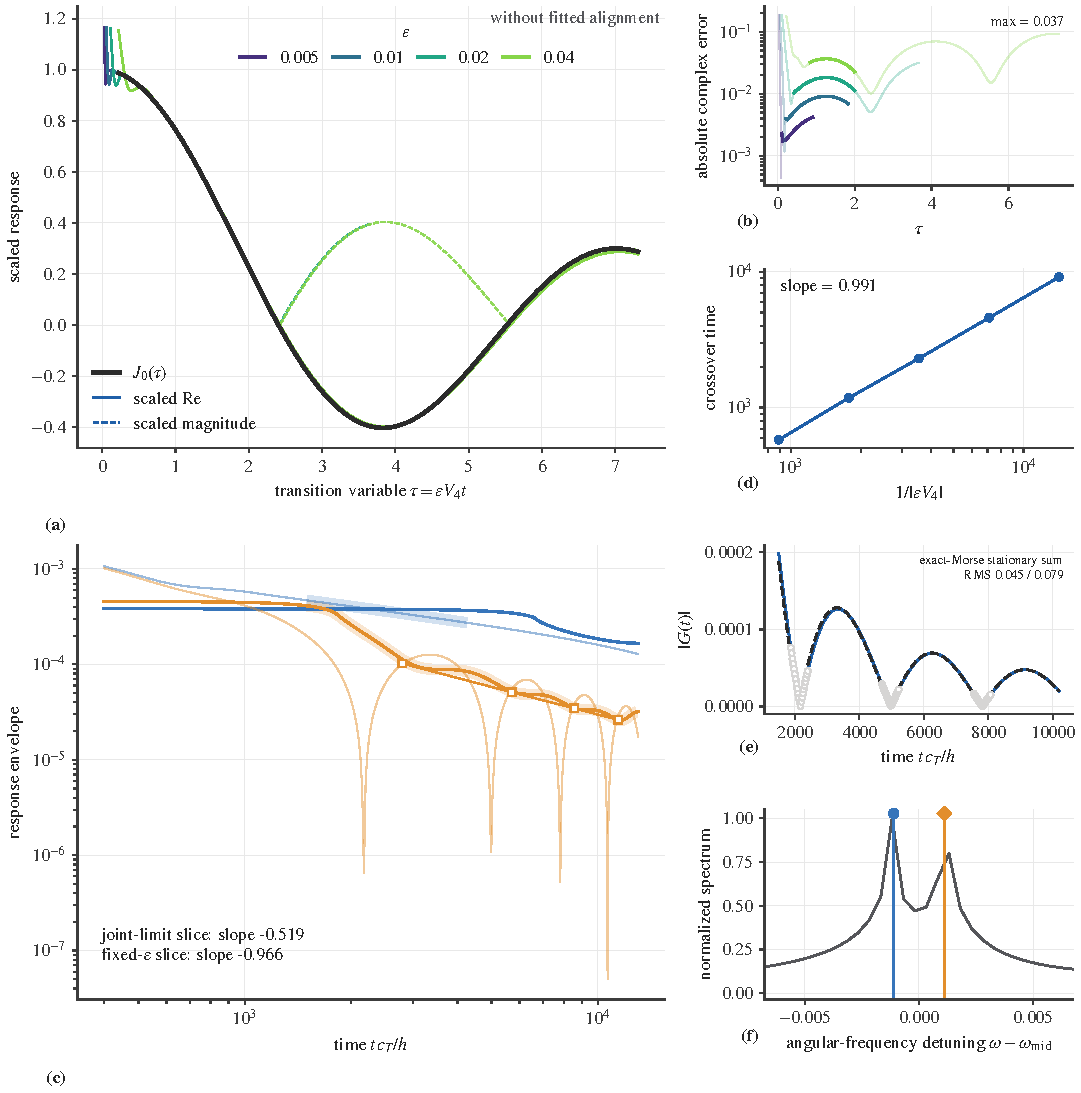
\includegraphics[width=\SixPanelFigureWidth]{../figures/main/figure_06_decay_crossover.pdf}
  \caption{\FigureSixCaption}
  \label{fig:decay-crossover}
\end{figure}

\subsection{Overlap with isolated stationary points}

Under the growing-\(\lvert\tau\rvert\) overlap conditions, but only while the
accumulated second- and higher-order phase corrections remain controlled, the
same branch entered the isolated-point scale
\(O(\lvert\varepsilon V_4\rvert^{-1/2}t^{-1})\).  This conclusion follows from the
independent growing-parameter stationary-phase argument in
Theorem~\ref{thm:growing-bessel-morse-overlap}; the compact-\(\tau\) theorem
cannot be extrapolated to large \(\lvert\tau\rvert\).  The limit and its
explicit error budget are stated in Eqs.~\eqref{eq:growing-overlap-limit}
and \eqref{eq:growing-overlap-error}, while
Eq.~\eqref{eq:bessel-overlap-response} restores the response normalization.
The overlap proof
directly resolves the alternating angular stationary points and recovers the
Cartesian minimum and saddle signature factors within the declared local
annulus.

Expanding the large-argument Bessel factor in this controlled overlap produced
the same coefficient and phases as the corresponding first-order
four-minimum/four-saddle Morse sum in
Eq.~\eqref{eq:bessel-morse-overlap}, not
merely the same decay exponent.  The fourfold multiplicity of each critical
family cancelled the angular-curvature factor, leaving the expected radial and
angular stationary-phase prefactor.  Away from destructive-cancellation times,
a fixed small nonzero \(\varepsilon\) slice has the \(t^{-1}\) time exponent.
Along a joint path, however, the prefactor
\(\lvert\varepsilon V_4\rvert^{-1/2}\) remains explicit and can diverge as the
ring is restored.  Root-mean-square binning is therefore the suitable
cancellation-safe observable.  Figure~\ref{fig:decay-crossover} presents two
numerical asymptotic slices rather than one time trajectory: a
small-perturbation joint-limit slice and a fixed-anisotropy slice.  The plotted
late bins and
\(\LateDecaySlope\) in Fig.~\ref{fig:decay-crossover}, however, belong to the
separate fixed-anisotropy endpoint discussed next; they are not a numerical
joint-path test of the growing-\(\lvert\tau\rvert\) theorem.  The connection
between the slices is the proved growing-\(\lvert\tau\rvert\) overlap above.

\subsection{Fixed-anisotropy Morse endpoint}

% Claim C7
At fixed nonzero anisotropy, and only for resolved nondegenerate critical
points away from the window boundary, standard two-dimensional stationary
phase applied to the exact full-wave Cartesian branch gave the endpoint in
Theorem~\ref{thm:fixed-anisotropy-decay}.  The signed Hessian sum in
Eq.~\eqref{eq:morse-stationary-sum} uses the exact critical frequencies,
modal amplitudes, and Cartesian determinants rather than their first-order
approximations.  It predicts a generic \(t^{-1}\) contribution to the
undoubled positive-frequency response from each nonnodal isolated point; the
physical real response is \(2\operatorname{Re}G^{+}\).  This use of standard
two-dimensional stationary phase follows established guided-wave asymptotics
\citep{velichko2007excitation,chapuis2010focusing,karmazin2013caustics}.

At fixed anisotropy, the full-wave response approached this
parameter-determined sum over the declared comparison window.  Its
root-mean-square envelope gave the slope \(\LateDecaySlope\), as shown in
Fig.~\ref{fig:decay-crossover}.  This endpoint complements the joint-limit
Bessel law: the former keeps \(\varepsilon\) fixed while time increases,
whereas the latter takes a controlled two-parameter limit.  The remainder
\(O_\varepsilon(t^{-2})\) in Eq.~\eqref{eq:morse-stationary-sum} is not uniform
as \(\varepsilon\to0\), so this endpoint does not replace the coalescing-ring
description.

\subsection{Frequency separation and modulation rate}

Within the fourfold family on the tracked branch, the exact minimum and saddle
frequencies appeared as two critical-frequency features of the infinite,
lossless continuum.  Their nonnegative separation in
Eq.~\eqref{eq:critical-frequency-separation} is twice the modulation
angular-frequency magnitude in Eq.~\eqref{eq:signed-modulation-rate}.  This
factor-of-two statement is restricted to the signed two-family modulation and
keeps the feature separation distinct from the magnitude that multiplies the
dimensionless time \(t\)
after the mean carrier has been removed.

At leading order, the separation is \(2\lvert\varepsilon V_4\rvert\), whereas
the modulation magnitude is \(\lvert\varepsilon V_4\rvert\).  The minimum and
saddle signature phases then generate the signed cosine recovered in the
growing-parameter overlap.  The quantitative comparison uses the exact
critical-point frequencies; the spectrum panel of
Fig.~\ref{fig:decay-crossover} is qualitative.  At fixed anisotropy, unequal exact amplitudes and
higher-order phase corrections may deform the cosine into a two-phasor
modulation, but they do not alter the definition of the exact
critical-frequency separation.
